\chapter{Literature Review}  \label{Chapter3} 
This chapter delves into the extensive literature surrounding isosurface extraction techniques. Isosurface extraction is pivotal in computer graphics, medical imaging, geophysics, and scientific visualization. The objective is to transform volumetric data into a visual representation, allowing a more intuitive understanding of the underlying information. Over the years, numerous algorithms and methodologies have been proposed, each with unique advantages and challenges. This chapter aims to comprehensively review these methods, focusing on their principles, algorithms, advantages, limitations, and applications. By the end of this chapter, readers should have a holistic understanding of the evolution and current state of isosurface extraction and mesh generation techniques.

\section{Marching Squares} \label{Marching-Squares}

Marching Squares (MS) is a contouring technique primarily used for 2D scalar fields. It is the 2D counterpart to the Marching Cubes algorithm (explained in detail in \ref{Marching-Cubes}), which operates in three dimensions. Marching Squares is primarily designed to derive contour lines, also known as isolines, from two-dimensional scalar fields. This technique is invaluable in various applications, ranging from creating topographic maps that represent terrain elevations to detecting contours in images, aiding in image analysis. By interpreting and visualizing data gradients, Marching Squares provides a clearer understanding of spatial variations and patterns, making it an essential tool in geospatial analysis, computer graphics, and digital image processing (\cite{Maple_2003}).

\vspace{2mm}
\subsection{Basic Principle}

The Marching Squares algorithm operates by dividing the 2D scalar field into a grid of squares. Each corner of these squares (or cells) is sampled to determine its scalar value. Based on these values, a specific configuration for the square is determined, which dictates how the contour line will pass through the square. Lookup tables are then employed to triangulate the square based on its configuration, resulting in a segment of the contour line.

\vspace{2mm}
\subsection{Algorithm Overview}

\begin{itemize}
\item \textbf{Grid Formation:} The 2D scalar field is divided into a grid of squares.

\item \textbf{Corner Sampling:} The scalar value at each corner of the square is determined, as denoted in Fig \ref{fig:Marching-Square-cell}.

\begin{figure}[H]
\centering
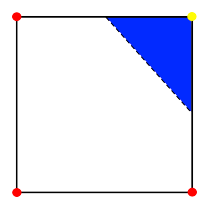
\includegraphics[height=0.3\textwidth,width=0.3\textwidth]{Figures/Marching-Sqaure-cell.png}
\decoRule
\caption{A marching square. The points at the corners denote the
sample points. Red points are outside the isoline and yellow point is inside the isoline. The dotted line marks the isoline, and the blue color defines the ’inside’} (\cite{Rassovsky_2014})
\label{fig:Marching-Square-cell}
\end{figure}

\item \textbf{Configuration Determination:} The four corners of each square provide \(2^4 = 16\) possible configurations, as displayed in Fig \ref{fig:Marching-Square-lookup-table}. With rotational and reflective symmetry, all possible combinations were reduced to 4 distinct configurations (Fig. \ref{fig:MS-4-unique-case}). A configuration for the square is identified Based on the scalar values at the corners and a specified isovalue.

\begin{figure}
\centering
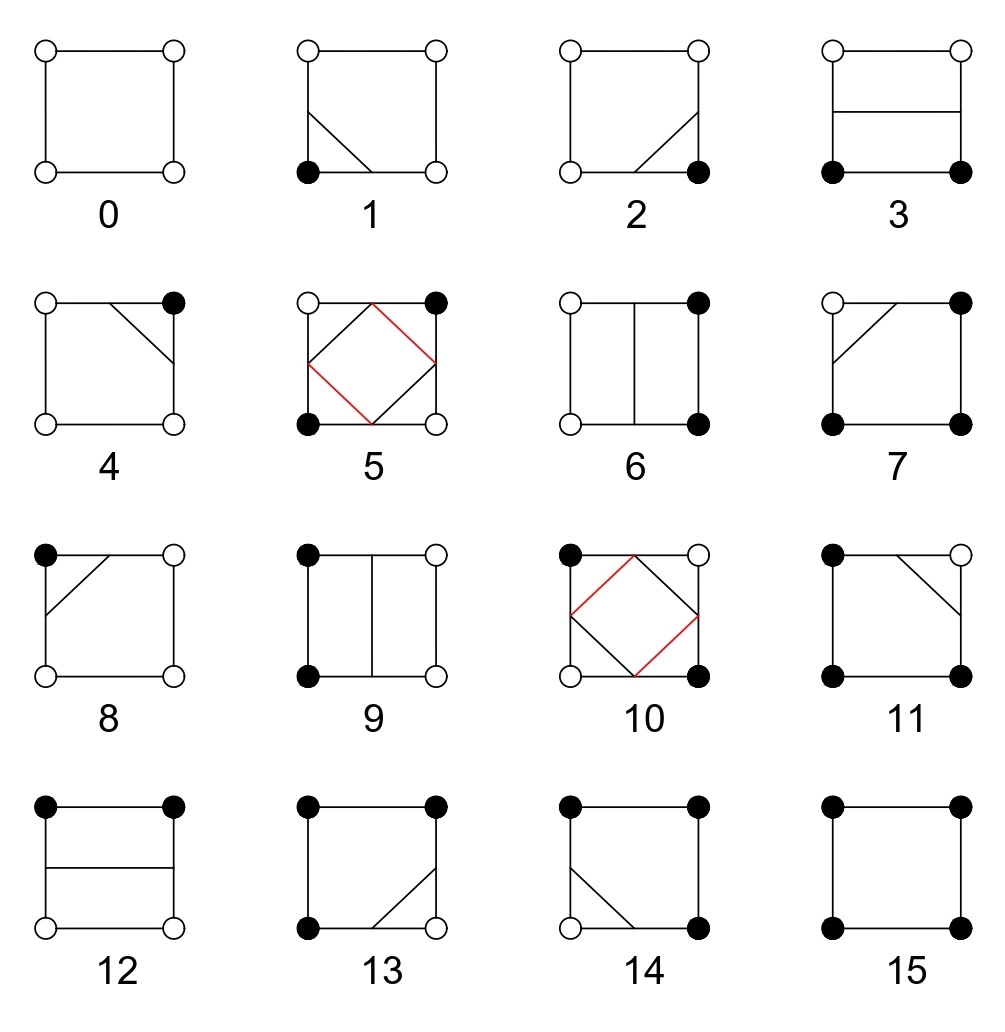
\includegraphics[width=0.85\textwidth]{Figures/Marching-Square-lookup-table.jpg}
\decoRule
\caption{The Marching Squares algorithm presents 16 configurations, with ambiguous scenarios evident in cases 5 and 10, highlighted by red lines.} (\cite{Rassovsky_2014})
\label{fig:Marching-Square-lookup-table}
\end{figure}

\begin{figure}
\centering
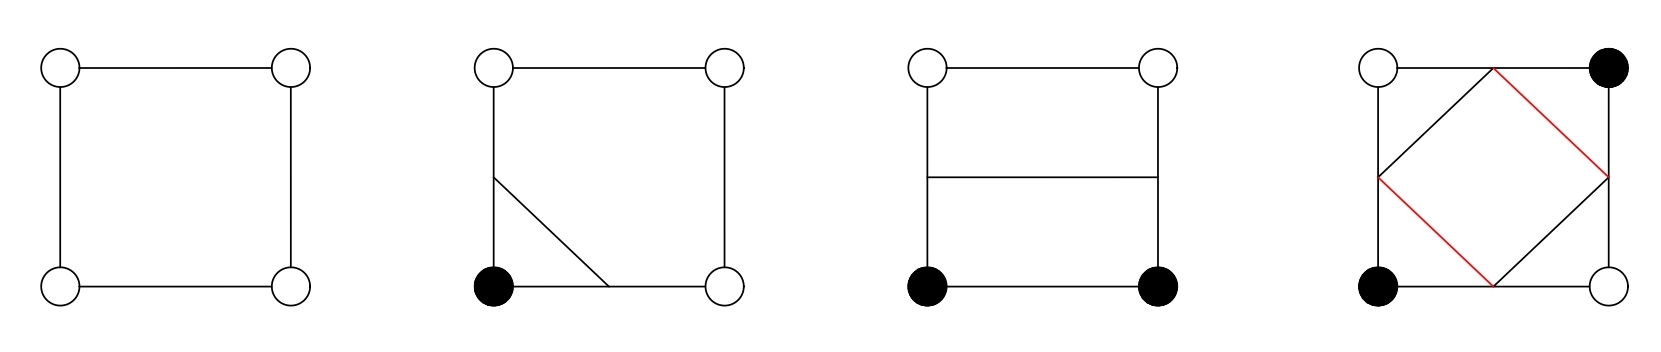
\includegraphics[width=0.90\textwidth]{Figures/MS-4-unique-case.jpg}
\decoRule
\caption{The 4 unique configurations of the Marching Squares algorithm, which are necessary to reproduce all others.} (\cite{Rassovsky_2014})
\label{fig:MS-4-unique-case}
\end{figure}

\item \textbf{Lookup Tables:} Using the determined configuration, lookup tables provide the necessary information to triangulate the square and extract the contour segment.

\item \textbf{Contour Construction:} The contour segments from each square are combined to form the complete contour line for the scalar field.
\end{itemize}

\subsection{Applications}

\begin{itemize}
\item \textbf{Robotic Manipulation:}
The fast marching square method, a variant of Marching Squares, has been employed in kinesthetic learning for robotic manipulation, allowing robots to learn from human demonstrations and adapt to their environment (\cite{Prados_2023}).

\item \textbf{Feature Preservation in 3D:}
The Marching Squares principle has been extended to 3D scenarios, as seen in the Cubical Marching Squares (CMS) algorithm, which aims to preserve sharp features in volumetric data (\cite{Chien-Chang_2005}).

\item \textbf{Topographic Mapping:} The algorithm is widely used in generating topographic maps, where contour lines represent constant elevation levels.

\item \textbf{Image Processing:}
Marching Squares can be used for image contour detection, aiding in object recognition and other image analysis tasks.
\end{itemize}

\subsection{Advantages}
\begin{itemize}
\item \textbf{Simplicity}: The algorithm is relatively straightforward to implement, especially compared to its 3D counterpart, Marching Cubes.
\item \textbf{Efficiency}: Marching Squares can quickly generate contour lines for large 2D scalar fields.
\end{itemize}

\subsection{Limitations}
\begin{itemize}
\item \textbf{Ambiguities}: When considering the problem in MS, there are two configurations, which could result in ambiguous topology. That is to say, the decision of which case should be used is undefined by the algorithm. Those cases, for the MS algorithm, are visible in Fig \ref{fig:ambiguity}.

\begin{figure}[H]
\centering
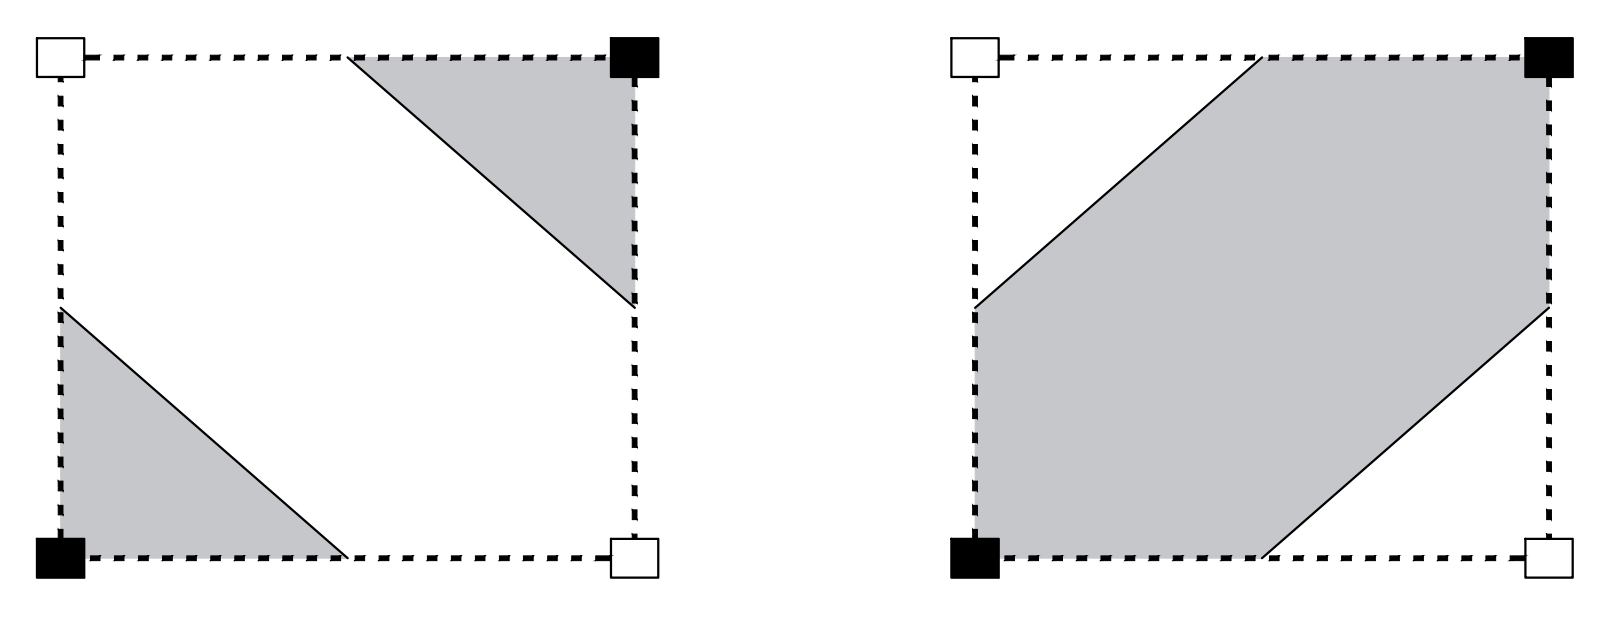
\includegraphics[height=0.26\textwidth,width=0.55\textwidth]{Figures/ambiguity.jpg}
\decoRule
\caption{The black corners are inside the surface. For this specific case, there are two possible configurations. This is then considered a face ambiguity.} (\cite{Chien-Chang_2005})
\label{fig:ambiguity}
\end{figure}

\item \textbf{Resolution Dependency}: The quality and accuracy of the extracted contour lines can be highly dependent on the resolution of the grid.
\end{itemize}

\section{Marching Cubes} \label{Marching-Cubes}

A crucial computer graphics method called Marching Cubes (MC) was created in 1987 by \cite{Lorensen_1987}. It is intended to produce a polygonal mesh representing an isosurface inside a 3D grid of data points and is often used in industries including geophysics, scientific visualization, and medical imaging. MC revolutionized these fields by transforming challenging scalar field data into intuitive 3D representations. It is necessary for portraying complicated structures, allowing scientists and medical practitioners to visualize and analyze data more comprehensibly and educationally, eventually improving diagnostic and research capacities and furthering our knowledge of complex phenomena (\cite{Lorensen_1987}).

\vspace{2mm}
\subsection{Basic Principle}

The fundamental concept of MC is to subdivide a 3D scalar field into a collection of tiny cubes, provided that a regular grid represents the field. The method selects the polygon(s) that correspond to the portion of the isosurface that traverses each cube.

\vspace{2mm}
\subsection{Algorithm Overview}

\begin{itemize}
\item \textbf{Cube classification:} Cube classification classifies a three-dimensional cube's interior according to the values assigned to each of its eight corners. 
Each corner may have a value that is either higher or lower than the isovalue, which leads to 256 different configurations. With rotational and reflective symmetry authors (\cite{Lorensen_1987}) reduced all possible combinations to these to 15 distinct configurations (Fig. \ref{fig:MC-15-cases}), making it easier to analyze and describe intricate 3D data structures.

\begin{figure}
\centering
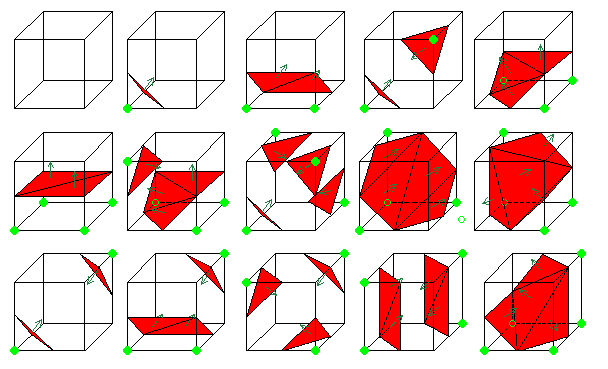
\includegraphics[height=0.6\textwidth,width=0.9\textwidth]{Figures/MC-15-cases.png}
\decoRule
\caption{Illustration of the 15 configurations of the marching cubes technique. The green vertices are the ones classified as “inside” the isosurfaces, whereas the remaining ones as “outside”.} (\cite{Lorensen_1987})
\label{fig:MC-15-cases}
\end{figure}
    

\item \textbf{Edge Intersection:}
The Marching Cubes algorithm works by dividing the volumetric dataset into small cubes. For each cube, the algorithm determines where the isosurface intersects the cube's edges. This is done by checking the scalar values at the cube's vertices against the isosurface's value. If one vertex is below the isosurface value and the other is above, the edge is intersected by the isosurface. The exact location of the intersection can be determined using linear interpolation between the two vertex values (\cite{Lorensen_1987}).
\item \textbf{Polygon Construction:}
Once the intersections are identified, the next step is constructing polygons that approximate the isosurface within the cube. This is typically done using a precomputed table, known as the edge or triangle table. This table provides a lookup for connecting the intersections based on the specific scalar values at the cube's vertices. The result is a set of triangles that approximate the isosurface within the cube (\cite{Lorensen_1987}).
\item \textbf{Mesh Generation:}
The ultimate 3D mesh representation of the isosurface is created during the "Mesh Generation" step of isosurface extraction. This stage merges the polygons produced from each cube in the volumetric dataset.  The mesh quality depends on the edge intersection calculations' accuracy and the polygons' correct construction. Once the mesh has been created, it may be displayed and altered for various uses, including computer graphics, medical imaging, and scientific visualization, giving essential insights into the underlying data (\cite{Wilhelms_1990}).
\end{itemize}

\subsection{Advantages}
\begin{itemize}
\item \textbf{Efficiency:} MC is relatively fast and can be applied to run in real-time for specific applications.
\item \textbf{Simplicity:} The algorithm is theoretically straightforward and relies on lookup tables for operation.
\end{itemize}

\subsection{Limitations} 
\begin{itemize}
\item \textbf{Ambiguities and Topological Errors:}
One of the most significant issues with the innovative Marching Cubes algorithm is the presence of unclear cases (Fig. \ref{fig:MC-ambiguity}). These ambiguities arise when the isosurface intersects the cube in a way that there are multiple conceivable ways to triangulate the intersected boundaries, leading to different topologies (\cite{Nielson_1991}).

\begin{figure}
\centering
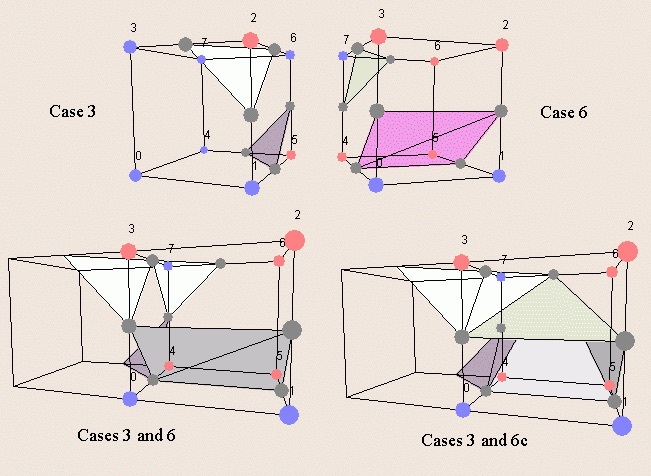
\includegraphics[height=0.55\textwidth,width=0.88\textwidth]{Figures/MC-Ambiguity-3D.jpeg}
\decoRule
\caption{An example of an ambiguous case in Marching Cubes, where case 3 and case 6 are incompatible.} (\cite{Lingrand_2003})
\label{fig:MC-ambiguity}
\end{figure}

To cope with these topology errors (as holes in the 3D model), 6 families, Fig. \ref{fig:MC-ambiguity-solution}, have been added to the marching cubes cases. These families have to be used as complementary cases. For instance, in the previous Fig. \ref{fig:MC-ambiguity}, case 6c must be used instead of the standard complementary of case 6 to avoid ambiguity.

\begin{figure}
\centering
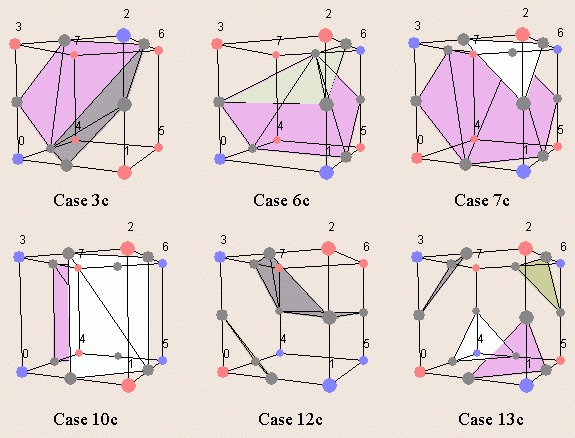
\includegraphics[height=0.65\textwidth,width=0.88\textwidth]{Figures/MC-Ambiguity-solution.jpeg}
\decoRule
\caption{An example of an added complementary cases in Marching Cubes} (\cite{Lingrand_2003})
\label{fig:MC-ambiguity-solution}
\end{figure}

This ambiguity can lead to crashes or holes in the generated surface, especially when neighboring cubes choose different triangulations. Solutions like the Asymptotic Decider (\cite{Nielson_1991}) and Extended Marching Cubes (\cite{Raman_2008}) have been proposed to address these ambiguities (Wang et al., 2020).

\item \textbf{Resolution Dependency:} The resolution of the input scalar field directly affects the quality of the extracted shallow. As displayed in Fig. \ref{fig:MC-sphere-ex} and Fig. \ref{fig:MC-diffrent-resolution}, it is important to note that finer details may be missed at lower resolutions, or the shallow may be excessively smoothed.

\begin{figure}
\centering
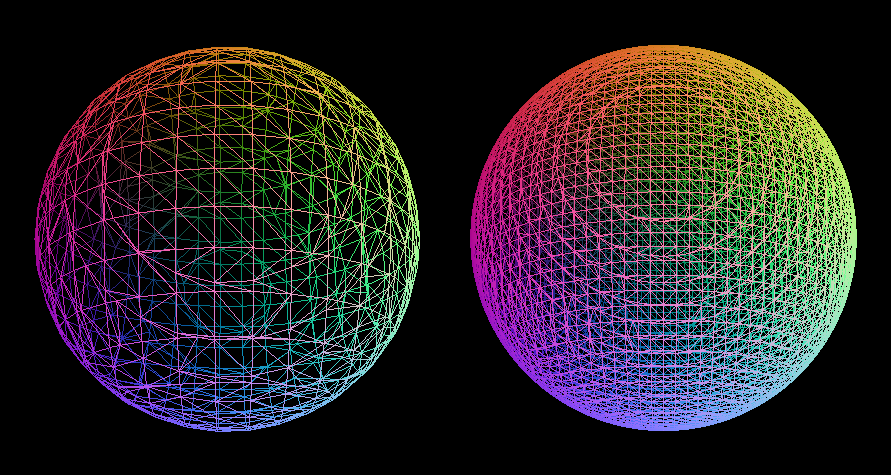
\includegraphics[height=0.5\textwidth,width=0.88\textwidth]{Figures/MarchingCubesSphere.png}
\decoRule
\caption{The comparison of surfaces extracted from the regular cube at two resolutions.} (\cite{Lingrand_2003})
\label{fig:MC-sphere-ex}
\end{figure}

\begin{figure}
\centering
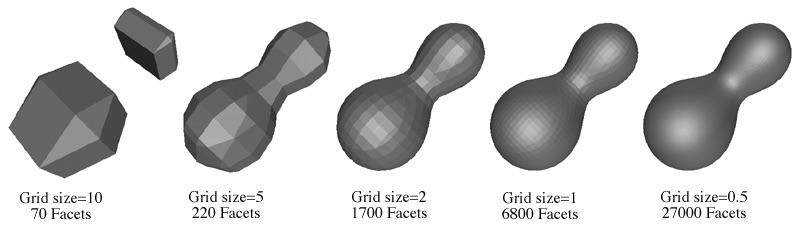
\includegraphics[height=0.3\textwidth,width=\textwidth]{Figures/MC-diffrent-resolution.jpeg}
\decoRule
\caption{The comparison of surfaces extracted at different resolutions. The low-resolution surface misses the finer details present in the high-resolution surface.} (\cite{Bourke_2023})
\label{fig:MC-diffrent-resolution}
\end{figure}

\item \textbf{Lack of Sharp Feature Preservation:} Marching Cubes tend to harvest rounded or smoothed surfaces, even if the original data has sharp features (Fig. \ref{fig:MC-loss-of-sharp-feature}). Methods like Feature-Preserving Marching Cubes have been proposed to address this issue (\cite{Chien-Chang_2005}).

\begin{figure}
\centering
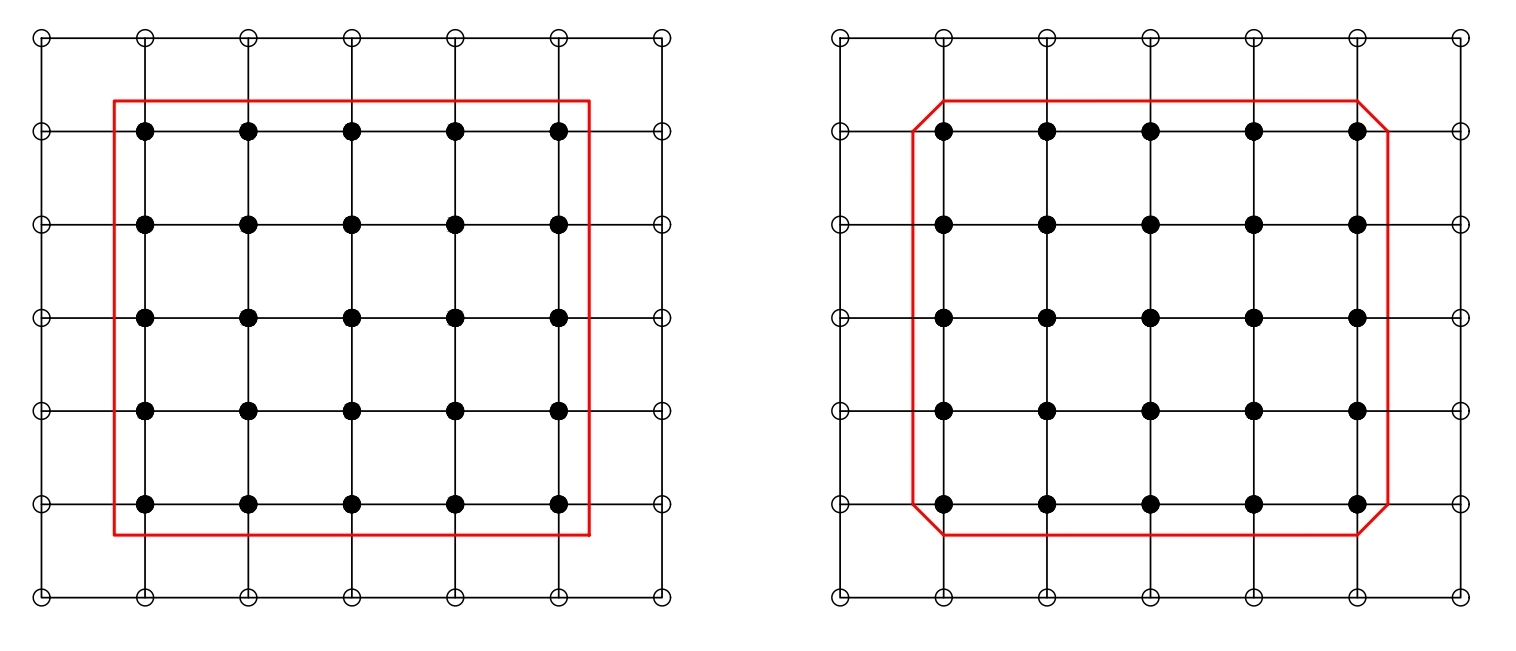
\includegraphics[height=0.45\textwidth,width=\textwidth]{Figures/MC-loss-of-sharp-feature.jpg}
\decoRule
\caption{A sharp feature in the data (left) gets smoothed out in the surface extracted by Marching Cubes (right).} 
\label{fig:MC-loss-of-sharp-feature}
\end{figure}

\end{itemize}

\subsection{Extensions and Variants} 

Over the years, several delays and variants of the MC algorithm have been planned to address its limitations. Some notable ones include Extended Marching Cubes (\cite{Raman_2008}), Asymptotic Decider (\cite{Nielson_1991}), and Dual Marching Cubes (\cite{Nielson_2004}).

\section{Dual Contouring} \label{Dual-Contouring}

Dual Contouring (DC) is an advanced isosurface extraction technique introduced by \cite{Ju_2002}. It was developed as an alternative to the MC algorithm to address some limitations, particularly in preserving sharp features and handling complex topologies. DC has found applications in various fields, including computer graphics, terrain modeling, and scientific visualization, where high-quality surface representations are essential.

\vspace{2mm}
\subsection{Basic Principle}

Unlike MC, which operates on the edges of the grid cells, DC focuses on the grid vertices. The algorithm generates a dual grid, where each cell contains a single vertex, representing the intersection of the isosurface with the cell. This approach allows for better representation of sharp features and complex topologies.

\vspace{2mm}
\subsection{Algorithm Overview}

\begin{itemize}
\item \textbf{Vertex Generation:} 
For each cell in the grid, if the cell intersects the isosurface, a vertex is generated. The optimal position of this vertex is determined by minimizing the Quadratic Error Function (QEF), which measures the error between the vertex position and the isosurface. The QEF is formulated as:
\begin{equation}
QEF(v) = \sum_{i} (n_i \cdot v - d_i)^2
\label{eq:qef}
\end{equation}
Where \( n_i \) is the normal to the isosurface at the \(i^{th}\) intersection point, \( v \) is the vertex position, and \( d_i \) is the signed distance from the origin to the isosurface along the normal \( n_i \) (\cite{Ju_2002}).

\item \textbf{Edge Construction:} Edges are constructed by connecting vertices in adjacent cells. This step ensures that the generated surface is manifold and has no gaps or holes.

\item \textbf{Polygon Construction:} After determining the optimal vertex positions within each cell using the QEF, the next step is connecting these vertices to form polygons representing the isosurface. In Dual Contouring, the polygons are typically quads (Fig. \ref{fig:DC-quad}), but they can be decomposed into triangles for compatibility with most graphics hardware. The connectivity is determined based on the topology of the isosurface intersections within each cell.

\begin{figure}[H]
\centering
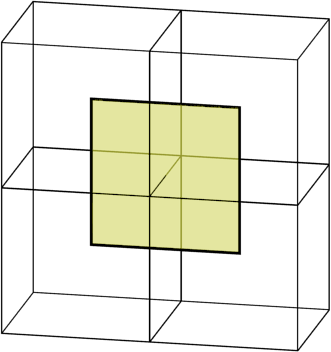
\includegraphics[height=0.5\textwidth,width=0.5\textwidth]{Figures/dc_single_face.png}
\decoRule
\caption{The face is associated with a single edge. It has a point in every adjacent cell.} (\cite{Boristhebrave_2018})
\label{fig:DC-quad}
\end{figure}

\item \textbf{Mesh Refinement:} The initial mesh generated by Dual Contouring might not always be of the desired quality, especially in regions with intricate features or noisy input data. Mesh refinement involves subdividing larger polygons, smoothing vertex positions (while still adhering to the isosurface), and removing artifacts. This step ensures the final mesh is visually appealing and topologically accurate (\cite{Schaefer_2007}).
\end{itemize}

\subsection{Advantages}
\begin{itemize}
\item \textbf{Sharp Feature Preservation:} DC excels in preserving sharp features in the data, which can be smoothed out by algorithms like MC. Figure \ref{fig:DC-MC-compare} shows sharp feature preservation compared to the MC algorithm.

\begin{figure}
\centering
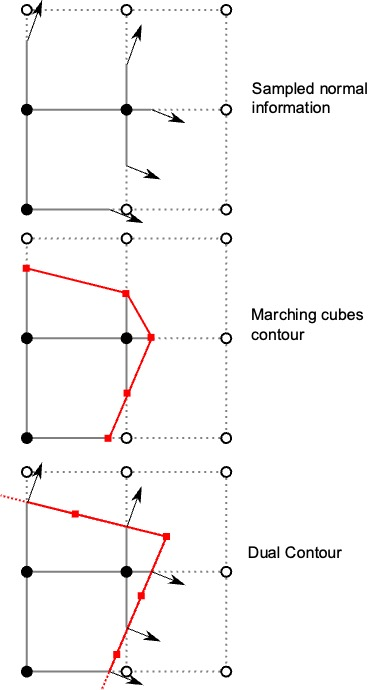
\includegraphics[height=0.95\textwidth, width=0.55\textwidth]{Figures/DC-MC-compare.jpg}
\decoRule
\caption{A signed grid with edge tagged by Hermite data (top), its MC contour (Middle), and its DC contour (bottom)}(\cite{Ju_2002})
\label{fig:DC-MC-compare}
\end{figure}

\item \textbf{Topological Flexibility:} DC can handle complex topologies, ensuring that the generated surface is manifold and does not have gaps or holes.
\end{itemize}

\subsection{Limitations}
\begin{itemize}
\item \textbf{Computational Complexity:} DC can be more computationally intensive than MC, especially for large datasets.

\item \textbf{Memory Consumption:} Due to the dual grid and additional data structures, DC can consume more memory than MC.

\item \textbf{Colinear normals:} 
As described in the original paper (\cite{Ju_2002}), the handling of the QEF is a significant limitation of the Dual Contouring algorithm. When solving the QEF, the aim is to find the point most consistent with the normals of the function. However, there's no guarantee that the resulting point will be inside the cell. As illustrated in Fig. \ref{fig:DC-colinear-ch3}, this issue becomes particularly pronounced in scenarios with large flat surfaces where all the sampled normals are identical or very similar. This issue is discussed extensively in Section \ref{challanges-QEF-minimization} of Chapter \ref{Chapter5}.

\begin{figure}
    \centering
    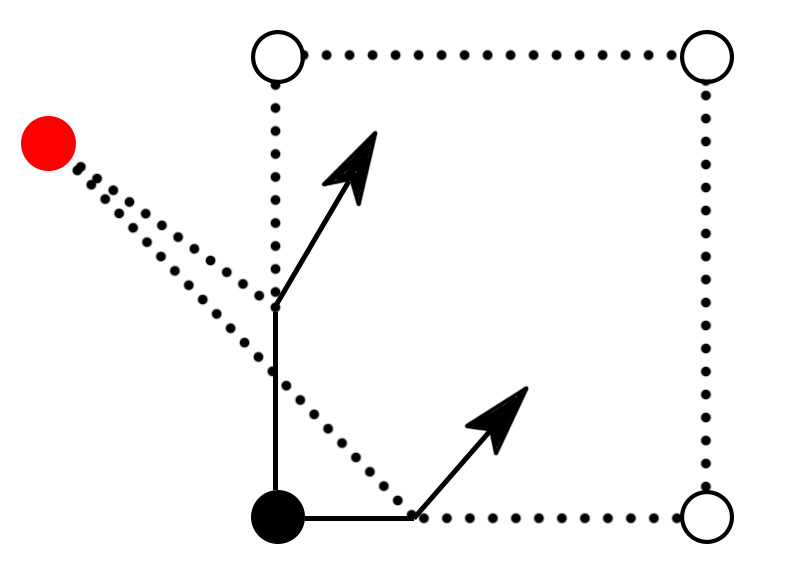
\includegraphics[width=0.4\textwidth]{Figures/DC-colinear.jpg}
    \decoRule
    \caption{Illustration of parallel normals due to a large flat surface.}(\cite{Boristhebrave_2018})
    \label{fig:DC-colinear-ch3}
\end{figure}

\item \textbf{Manifold:} 
While a mesh generated by dual contouring is always watertight, it doesn't always result in a well-defined surface. Given that, there's only one point per cell, situations where two surfaces pass through a single cell will result in them sharing that cell. This phenomenon leads to what's known as a "non-manifold" mesh (Fig. \ref{fig:DC-manifold}). 

\begin{figure}
\centering
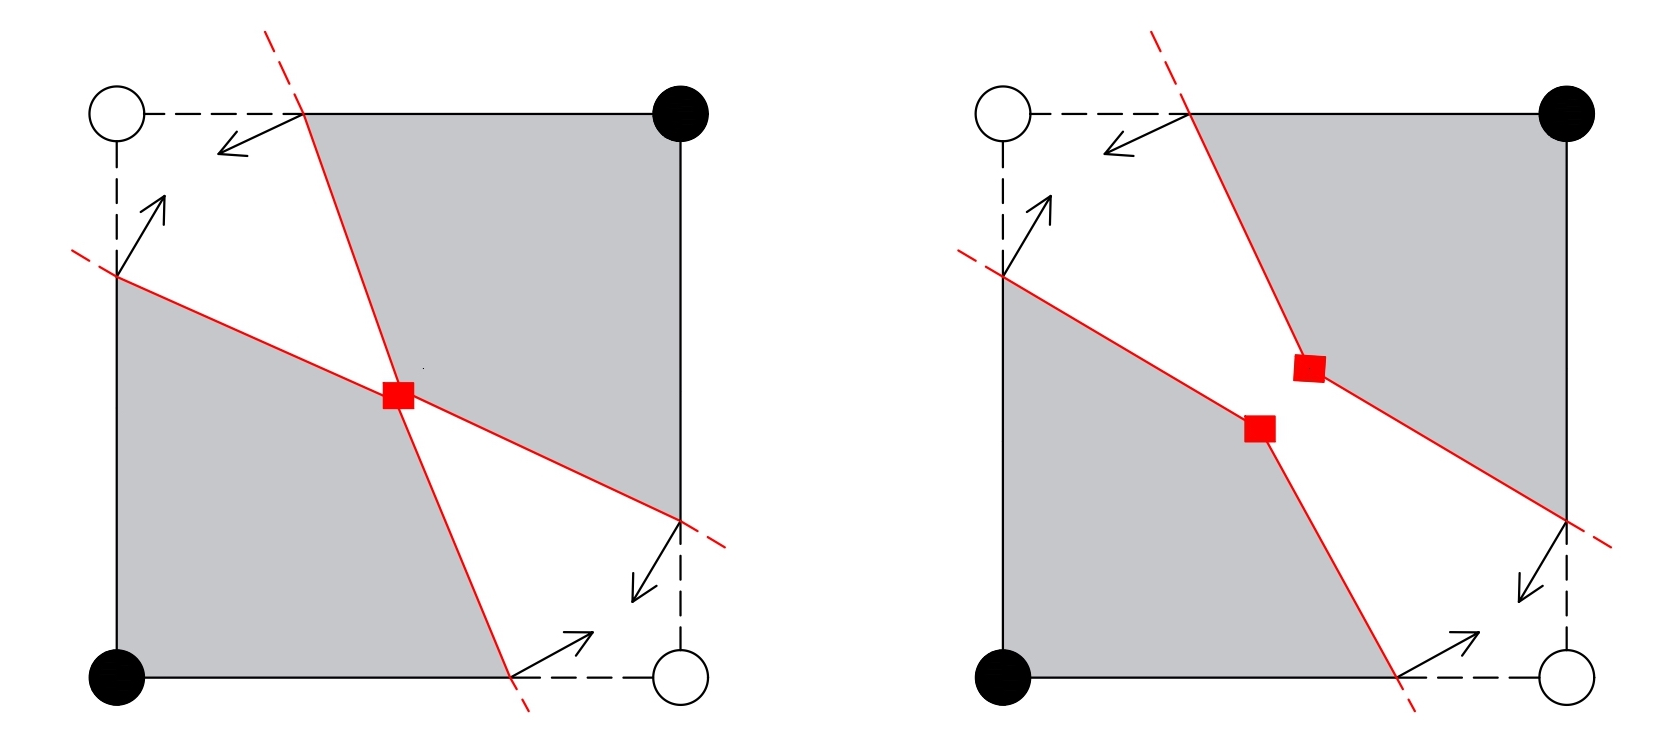
\includegraphics[width=0.7\textwidth]{Figures/DC-manifold.jpg}
\decoRule
\caption{A limitation of the DC algorithm is that it permits only one point per cell (left). An optimal solution for a given scenario would require two vertexes (right).}(\cite{Boristhebrave_2018})
\label{fig:DC-manifold}
\end{figure}

Non-manifold meshes can interfere with certain texturing algorithms and are particularly prevalent in scenarios where solids are thinner than the cell size or when multiple objects are in close proximity to each other (\cite{Schaefer_2007}).

\item \textbf{Mesh Quality:} While DC preserves sharp features, it can sometimes produce jagged or noisy surfaces, especially if the input data is not clean or well-sampled (\cite{Zhang_2004}).

\item \textbf{Inability to Generate Thin Features:} As illustrated in Fig. \ref{fig:DC-thin-brick} and Fig. \ref{fig:DC-think-brick-mesh}, one of the main limitations of DC is its difficulty in generating thin features in the mesh. This limitation arises because the dual contouring algorithm only allows one vertex per cell, which inherently restricts the representation of thin structures. This can lead to a loss of detail in specific datasets where thin structures are crucial (\cite{Zhang_2004}).

\begin{figure}
\centering
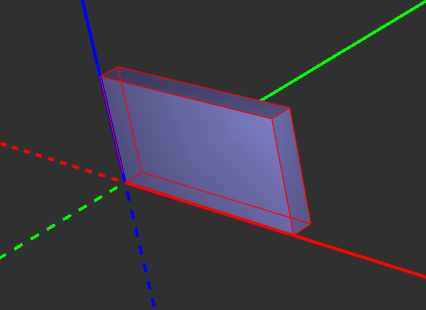
\includegraphics[height=0.7\textwidth, width=0.8\textwidth]{Figures/Thin-brick.png}
\decoRule
\caption{Analyzing the DC algorithm when the object's width is smaller than the width of the cell.}
\label{fig:DC-thin-brick}
\end{figure}

\begin{figure}
\centering
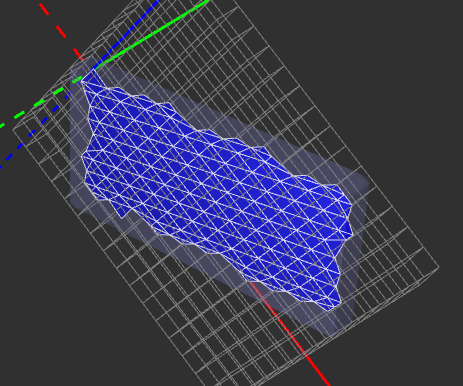
\includegraphics[height=0.7\textwidth, width=0.8\textwidth]{Figures/DC-thin-brick-mesh.png}
\decoRule
\caption{As a consequence, the DC algorithm fails to produce thin features, leading to the generation of infinitely thin sheet.}
\label{fig:DC-think-brick-mesh}
\end{figure}
\end{itemize}

\subsection{Extensions and Variants}

Several extensions and variants of the DC algorithm have been proposed to address its limitations and improve its performance. Notable ones include Adaptive Dual Contouring, Simplified Dual Contouring, and Feature-Preserving Dual Contouring (\cite{Zhang_2004}).

\section{Cubical Marching Squares} \label{Cubical-Marching-Squares}

The Cubical Marching Squares (CMS) algorithm, as introduced by \cite{Chien-Chang_2005}, represents an evolution of the Marching Squares and Marching Cubes algorithms. Designed to extract isosurfaces from 3D scalar fields, CMS emphasizes adaptability and feature preservation, making it a significant advancement in the field of isosurface extraction.

\vspace{2mm}
\subsection{Basic Principle}

The Cubical Marching Squares (CMS) algorithm enhances traditional isosurface extraction techniques, aiming to represent a three-dimensional scalar field as a two-dimensional isosurface. Building on the principles of Marching Cubes, CMS introduces adaptability. Rather than uniformly processing the scalar field, it adjusts its resolution based on data complexity. This ensures that intricate features are captured in detail while simpler areas are efficiently processed, making CMS adept at producing detailed and accurate representations of 3D scalar fields (\cite{Chien-Chang_2005}).

\vspace{2mm}
\subsection{Algorithm Overview}

The Cubical Marching Squares (CMS) algorithm is a methodical process that combines the principles of Marching Squares and Marching Cubes (\cite{Lorensen_1987}), refining them with an adaptive approach to better capture the intricacies of 3D scalar fields. Here's a more detailed breakdown:

\begin{itemize}
\item \textbf{Initialization:}
The CMS algorithm initiates by segmenting the 3D scalar field into a grid of cubes reminiscent of the Marching Cubes approach. Each corner of these cubes undergoes sampling to ascertain their scalar values.

\item \textbf{Adaptive Subdivision:}
Diverging from the uniform operation of traditional Marching Cubes, CMS evaluates the variance of scalar values within each cube. When this variance exceeds a predefined threshold, signaling the presence of a potential feature or sharp transition, the cube is subjected to subdivision. This recursive adaptive process continues until the variance within each subdivided cube either falls below the threshold or reaches a predetermined maximum subdivision level (\cite{Chien-Chang_2005}).

\item \textbf{Feature Preservation:}
The algorithm calculates the gradient at each corner for each cube (or subdivided cube), approximating the surface normal. These normals are crucial in determining the optimal position of the vertex within the cube, ensuring that sharp features are well-represented.

\item \textbf{Lookup Tables and Vertex Positioning:}
A specific configuration is identified based on the scalar values at the corners of each cube. Using this configuration, the algorithm employs a lookup table to determine how the cube should be triangulated.

\item \textbf{Edge Construction and Isosurface Generation:}
As illustrated in Fig. \ref{fig:CMS}, a cube possesses six faces. The isocurve or the isosurface is generated using the Marching Cubes algorithm for each face. The isocurve produced consists of multiple segments for each face. Components akin to the MC are obtained when these segments are properly connected and reverted to the original cube. Edges are formed by linking vertices in adjacent cubes, serving as the foundation for the isosurface construction.

\begin{figure}
\centering
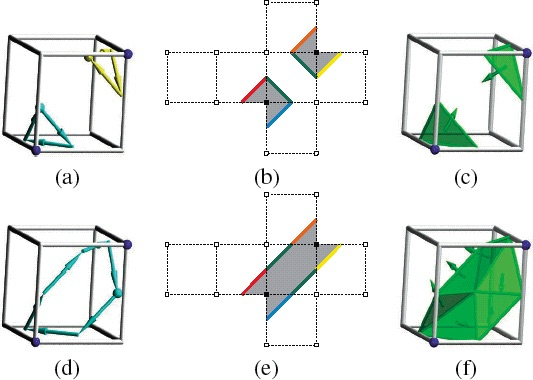
\includegraphics[width=0.85\textwidth]{Figures/CMS.jpeg}
\decoRule
\caption{Cubical Marching Squares illustration. A cube (a, d) unfolds into six squares (b, e). Each square is processed, and segments are returned to 3D to form components (a, d). Ambiguities are resolved in 2D, and the components are triangulated to form the isosurface (c, f).}(\cite{Chien-Chang_2005})
\label{fig:CMS}
\end{figure}

\item \textbf{Polygon Construction and Triangulation:}
The process of refining the isosurface involves triangulation. While the method chosen for triangulation can vary, it must remain consistent throughout the process. The term "cubical marching squares" arises from the ability to convert a single lookup table used in the Marching Cubes algorithm into six separate lookup tables used in the Marching Squares algorithm. While Marching Squares may be slower than Marching Cubes, it eliminates dependencies between cells by focusing on sharp features on the faces of cubes (\cite{Sreeparna_2017}).

\begin{figure}
\centering
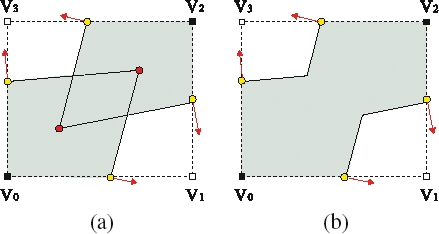
\includegraphics[width=0.75\textwidth]{Figures/CMS-Ambiguty.jpg}
\decoRule
\caption{A cell face that has intersecting sharp features. Self-intersection (a) should not happen in a volume; therefore, the algorithm chooses the correct disambiguated configuration (b) with preserved sharp features.}(\cite{Chien-Chang_2005})
\label{fig:CMS-Ambiguity}
\end{figure}

Challenges arise when determining the relationship between two components based solely on the signs of their vertices, leading to internal ambiguities. These ambiguities, which resemble face ambiguities, can be addressed using 3D sharp features. If two components have overlapping volumes, they are deemed connected; if not, they are treated as separate entities (Fig. \ref{fig:CMS-Ambiguity}). For each separate component, a triangle fan is constructed. In cases where two components are interconnected, the resulting surface takes on a cylindrical shape. For these scenarios, employing a dynamic programming approach is effective for triangulation and connecting components to create the final surface (\cite{Sreeparna_2017}).
\end{itemize}

\subsection{Advantages}
\begin{itemize}
\item \textbf{Higher Quality Meshes:} The adaptive nature of CMS allows for the production of meshes that more accurately represent the underlying scalar field, especially in regions with sharp features. Its flexibility ensures superior quality representations, giving it a distinct advantage over traditional methods.
\item \textbf{Efficiency:} As noted by \cite{Chien-Chang_2005}, CMS often generates fewer triangles than conventional Marching Cubes while achieving a similar or even superior level of detail, thanks to its adaptive subdivision of the scalar field.
\end{itemize}

\subsection{Limitations}
\begin{itemize}
\item \textbf{Complexity:} The algorithm's adaptive nature and the enhanced lookup tables introduce a higher complexity level than the traditional Marching Cubes.
\item \textbf{Ambiguities:} While CMS addresses many of the topological ambiguities inherent in Marching Cubes, certain configurations can still pose challenges. These ambiguities, discussed in the context of Marching Cubes by \cite{Nielson_1991}, continue to concern advanced algorithms like CMS.
\end{itemize}

\subsection{Applications}

Owing to its capability to capture sharp features and adapt to the underlying data, CMS has been employed in areas demanding high-quality surface representations. These include medical imaging, geophysics, and scientific visualization.


\section{Dual Marching Cubes} \label{Dual-Marching-Cubes}

The Dual Marching Cubes (DMC) algorithm, introduced by \cite{Nielson_2004}, is an evolution of the Marching Cubes and Dual Contouring algorithms. It aims to combine the strengths of both methods to produce high-quality isosurfaces from 3D scalar fields. The DMC algorithm is mainly known for its ability to generate adaptive and topologically accurate meshes, making it a significant advancement in the realm of isosurface extraction.

\vspace{2mm}
\subsection{Basic Principle}

DMC operates by constructing a dual grid from the original scalar field grid. Each cell corresponds to a vertex in the original grid in this dual grid. The algorithm generates vertices at optimal positions within each voxel of the dual grid, ensuring that the resulting mesh closely adheres to the underlying scalar field. By combining the adaptability of Dual Contouring with the robustness of Marching Cubes, DMC aims to produce isosurfaces that are detailed and topologically accurate (\cite{Schaefer_2004}).

\vspace{2mm}
\subsection{Algorithm Overview}

The Dual Marching Cubes algorithm is an advanced method that builds upon the principles of Marching Cubes but operates on a topologically dual grid to the structured grids used by other techniques. It aims to generate a mesh that closely represents the underlying scalar field while ensuring topological accuracy and adaptability. Here is a more detailed breakdown:

\begin{itemize}
\item \textbf{Initialization and Dual Grid Construction:}
The algorithm begins with a structured grid, often referred to as the Primal grid, that adaptively samples the function. From this primal grid, a dual grid is derived. The vertices of the dual grid are determined by the Quadratic Error Function calculations, pinpointing the features within each grid cell. This dual grid aligns with the function's features, and the surface is subsequently generated using a generalized version of Marching Cubes (\cite{Schaefer_2004}).

\begin{figure}[H]
\centering
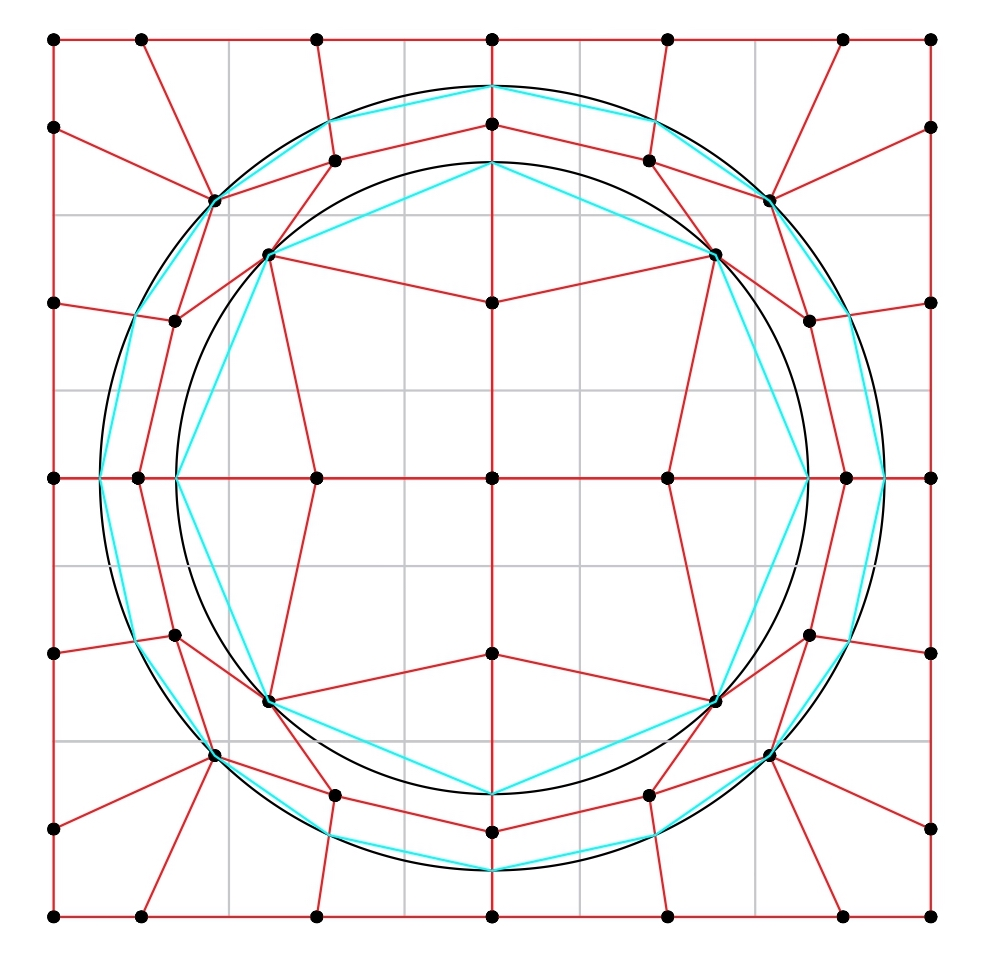
\includegraphics[height=0.75\textwidth,width=0.8\textwidth]{Figures/DMC-dual-grid.jpg}
\decoRule
\caption{2D visualization of the Dual Marching Cubes Algorithm on a thin torus}
\label{fig:DMC-dual-grid-ex}
\end{figure}

In the illustrated Fig. \ref{fig:DMC-dual-grid-ex}, the dual grid's formation in the Dual Marching Cubes algorithm is highlighted. The primal grid is shown in light grey, and the dual grid, constructed by connecting the QEF points, is emphasized in contrasting red. These QEF points are marked as black vertices. A comprehensive understanding of the dual grid's role and importance in the DMC algorithm can be found in Chapter \ref{Chapter6}.

\item \textbf{Scalar Field Analysis:}
Before diving into vertex generation, the algorithm analyzes the scalar field within each voxel. This involves determining if the voxel intersects the isosurface by checking if the scalar values at its corners span the desired isovalue. If an intersection is detected, the voxel is flagged for further processing.

\item \textbf{Feature Isolation and Vertex Generation:}
The Quadratic Error Function is used to determine the vertex that approximates the feature of the function inside a cell. This QEF is generated by computing tangent planes to the graph of the function on a grid of points sampled over the cell. The QEF is then minimized over the cell to find the vertex of the dual grid.

\item \textbf{Topology Creation:}
Once a grid is established and feature isolation generates the vertices of the dual grid, the next step is to generate the topology of the dual grid. This dual grid is topologically dual to the primal grid. A cell in the dual grid is created for every vertex in the grid. The vertices of this cell are the feature vertices inside each cube in the grid containing that vertex (\cite{Schaefer_2004}).

\item \textbf{Polygon Construction and Triangulation:}
After the topology creation, the algorithm forms polygons representing the isosurface. In DMC, these polygons are typically quads. However, these quads can be further divided into triangles for compatibility with most graphics hardware. The triangulation is guided by the scalar values at the voxel corners and the topology of the isosurface intersections within each voxel.

\item \textbf{Mesh Refinement and Post-processing:}
While topologically accurate, the initial mesh generated by DMC might require further refinement to enhance its visual quality. This involves subdividing larger polygons, smoothing vertex positions, and removing artifacts. The refinement ensures the final mesh is topologically accurate and visually appealing, making it suitable for various applications.
\end{itemize}

\vspace{2mm}
\subsection{Advantages}
\begin{itemize}
\item \textbf{Sharp Feature Preservation:} One of the standout features of DMC is its ability to reproduce sharp features such as edges and corners. Traditional methods might smooth out or miss these features, but DMC, by aligning vertices with the features of the implicit function, ensures that these sharp features are accurately represented in the generated mesh (Fig. \ref{fig:DMC}).

\item \textbf{Efficient Representation of Thin Structures:} DMC excels in representing both thin-walled structures and intricate thin features, as evident in Fig. \ref{fig:DMC}. Compared to other methods, DMC can generate a polygonal approximation with significantly fewer polygons, making it particularly advantageous for scenarios where the thickness or fineness of structures is a critical factor (Fig. \ref{fig:DMC-compare}). This capability ensures that both large-scale thin walls and minute details are captured without the need for excessive grid subdivision, a challenge that other algorithms might struggle with or require a much finer grid to address (\cite{Schaefer_2004}).

\begin{figure}
\centering
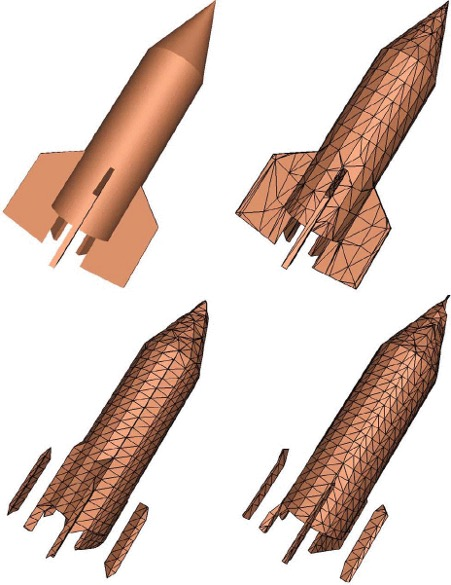
\includegraphics[height=0.6\textwidth, width=0.6\textwidth]{Figures/DMC.jpg}
\decoRule
\caption{CSG model of a rocket (upper left) and models approximating the shape using the same number of polygons. Dual Marching Cubes (upper right), Marching Cubes (lower left), and Dual Contouring (lower right).}(\cite{Schaefer_2004})
\label{fig:DMC}
\end{figure}

\begin{figure}[t]
\centering
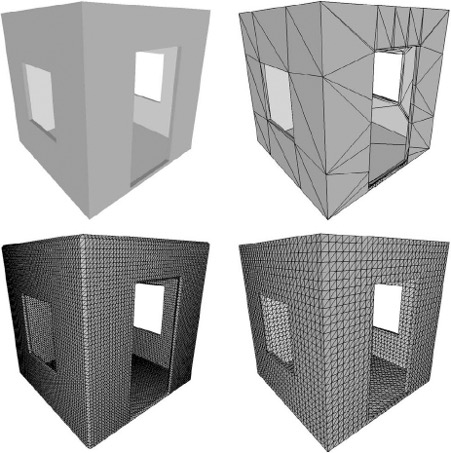
\includegraphics[height=0.6\textwidth, width=0.6\textwidth]{Figures/DMC-compare.jpg}
\decoRule
\caption{A thin-walled room defined via CSG (upper left). Polygonal approximations were generated by Marching Cubes (lower left, 67K polys), Dual Contouring (lower right, 17K polys), and Dual Marching Cubes (upper right, 440 polys). Using Dual Marching Cubes, the size of the contour mesh is insensitive to the thickness of the walls}(\cite{Schaefer_2004})
\label{fig:DMC-compare}
\end{figure}

\item \textbf{Topological Accuracy:} DMC ensures the generated mesh is topologically manifold, free from gaps, holes, or inconsistencies. This is crucial for many applications, especially in scientific visualization and computer graphics.

\item \textbf{Crack-free Mesh:} The algorithm ensures that the generated mesh is crack-free, eliminating the common problem of small gaps or inconsistencies that can arise in mesh generation.

\item \textbf{Scalability:} DMC is designed to handle large datasets efficiently, making it suitable for applications that deal with extensive volumetric data, such as medical imaging or geological studies.
\end{itemize}

\subsection{Limitations}

\begin{itemize}
\item \textbf{Computational Intensity:} One of the primary limitations of DMC is its computational demand. The algorithm can be computationally heavy, especially when aiming to capture intricate details and sharp features. This might lead to longer processing times, especially for large datasets.

\item \textbf{Complex Implementation:} The DMC algorithm, focusing on capturing sharp and thin features, can be more complex than traditional Marching Cubes. This complexity can pose developers challenges and lead to potential bugs if not implemented carefully.

\item \textbf{Dependency on Quality of Input Data:} The accuracy and quality of the generated mesh heavily depend on the quality of the input scalar field. Noisy or imprecise data can lead to sub-optimal results.

\item \textbf{Difficulty in Real-time Applications:} Due to its computational demands, using DMC in real-time applications, such as games or interactive simulations, can be challenging.

\item \textbf{Optimization Challenges:} While DMC aims to minimize errors using Quadratic Error Functions, finding the global minimum can be challenging, and the algorithm might sometimes settle for local minima, leading to sub-optimal vertex placements.
\end{itemize}

\subsection{Applications}

DMC's ability to produce detailed and topologically accurate isosurfaces has led to its adoption in various fields requiring high-quality surface representations. These include medical imaging, geophysics, and scientific visualization.

\section{Comparative Analysis of Methods}

This section will compare the discussed isosurface extraction methods, namely Marching Squares (MS), Marching Cubes (MC), Dual Contouring (DC), Cubical Marching Squares (CMS), and Dual Marching Cubes (DMC), based on various criteria.

\noindent \textbf{Mesh Quality:}
\begin{itemize}
\item \textbf{MS:} Provides a straightforward representation exclusively for 2D scalar fields. With the integration of a quadtree structure, it can adeptly capture intricate details.
\item \textbf{MC:} Produces a consistent mesh but often lacks in preserving sharp features. The mesh quality directly depends on the resolution of the input scalar field.
\item \textbf{DC:} Known for preserving sharp features, but the calculation for QEF can be tricky and cannot reproduce the thin features.
\item \textbf{CMS:} Produces high-quality meshes, especially in regions with sharp features, due to its adaptive nature.
\item \textbf{DMC:} Generates meshes closely representing the underlying scalar field, ensuring detail, topological accuracy, and the ability to represent thin surfaces or features that other methods might miss.
\end{itemize}

\noindent \textbf{Computational Efficiency:}
\begin{itemize}
\item \textbf{MS:} Efficient for 2D datasets with regular grid, but might require more computational resources when adapted for quadtree implementation.
\item \textbf{MC:} Relatively fast and can be applied in real-time for specific applications.
\item \textbf{DC:} More computationally intensive than MC due to QEF calculations, especially for large datasets.
\item \textbf{CMS:} Efficient in producing fewer triangles than MC for a similar level of detail.
\item \textbf{DMC:} While efficiently capturing details, it can be computationally demanding due to the dual grid construction and QEF minimization.
\end{itemize}

\noindent \textbf{Topological Accuracy:}
\begin{itemize}
\item \textbf{MS:} It ensures topological accuracy within 2D domains, faithfully representing the contours of scalar fields.
\item \textbf{MC:} Recognized for its inherent ambiguities, the method often encounters challenges in accurately representing complex topologies. These ambiguities can manifest as inconsistencies in the mesh. 
\item \textbf{DC:} Handles complex topologies well, ensuring the generated surface is manifold.
\item \textbf{CMS:} Addresses many topological ambiguities inherent in MC but still has some challenges.
\item \textbf{DMC:} Ensures topological accuracy by focusing on the dual grid, making it robust against topological errors and adept at representing thin features.
\end{itemize}

\noindent \textbf{Adaptability:}
\begin{itemize}
\item \textbf{MS:} It is designed exclusively for 2D fields, so its adaptability is confined to this dimension.
\item \textbf{MC:} Processes the scalar field uniformly, leading to potential loss of detail in complex regions.
\item \textbf{DC:} Focuses on grid vertices, allowing for better representation of sharp features.
\item \textbf{CMS:} Highly adaptive, adjusting its resolution based on data complexity.
\item \textbf{DMC:} Combines the strengths of MC and DC, ensuring adaptability, detail preservation, and the unique capability to represent thin surfaces or features.
\end{itemize}

\section{Summary}
Isosurface extraction is a pivotal technique in computer graphics, medical imaging, geophysics, and scientific visualization. The methods discussed in this chapter, namely Marching Cubes, Dual Contouring, Cubical Marching Squares, and Dual Marching Cubes, offer unique advantages and have specific limitations (Table \ref{table:comparison-of-methods}). 

\renewcommand{\arraystretch}{1.5}
\begin{table}[H]
\centering
\begin{tabular}{l|c|c|c|c|c}
 & MS & MC & DC & CMS & DMC \\
\hline
Easy to Implement & $\checkmark$ $\checkmark$ & - & - & - & - \\
Local Independence & $\checkmark$ & $\checkmark$ & - & $\checkmark$ & - \\
Smooth & - & $\checkmark$ & $\checkmark$ & $\checkmark$ & $\checkmark$ \\
Adaptive & - & - & $\checkmark$ & $\checkmark$ & $\checkmark$ \\
Minimize slivers & $\checkmark$ & - & $\checkmark$ & $\checkmark$ & $\checkmark$ \\
Sharp features & - & - & $\checkmark$ & $\checkmark$ & $\checkmark$ \\
Thin features & - & - & - & $ \sim $ & $\checkmark$ \\
\end{tabular}
\caption{Comparison of methods based on criteria. \\
$ \sim $  CMS is capable of representing thin features when utilized with octree adaptation and a grid of sufficiently fine resolution.
} \label{table:comparison-of-methods}
\end{table}

Marching Cubes, being one of the earliest methods, laid the foundation for isosurface extraction. However, its inability to preserve sharp features and handle complex topologies led to the development of advanced techniques like Dual Contouring and Cubical Marching Squares. Dual Contouring, while excelling at preserving sharp features, struggles with producing thin features and can be computationally intensive. On the other hand, Cubical Marching Squares introduces adaptability, ensuring detailed representation in complex regions while efficient in simpler areas. Dual Marching Cubes combines the strengths of both MC and DC, ensuring detail preservation, topological accuracy, and the capability to represent thin features that Dual Contouring lacks.

Choosing the right method depends on the application's specific requirements, the nature of the data, and the computational resources available. As research progresses in this domain, we can expect further refinements and new techniques that address the existing limitations and offer even more accurate and efficient isosurface extraction methods.